\chapter{Enhedstest af Wifi-klassen}
\label{appendix:BilagEnhedstestWifi}

For at teste Wifi-klassen anvendes to virtuelle maskiner, én til PC og én til Kontrolenheden, med en forbindelse, der simulerer Wifi-forbindelsen. 
Til testen opsættes tre test cases, som skal gennemføres før klassen kan godkendes, disse er som følgende:
	
	\begin{enumerate}
	\item Skal kunne oprette en TCP-forbindelse mellem to maskiner.
	\item Skal kunne sende en besked fra en maskine som kan læses på den anden.
	\item Socketen må ikke tilgås før der er oprettet forbindelse.
	\end{enumerate}
	
Til at teste Wifi-klassen er der oprettet projektet "Wifi test".
Forløbet i test main.cpp filen er som følgende:
	\begin{itemize}
	\item Opretter to tråde: en til at læse fra wifi og en til at skrive til wifi.
	\item Sende tråden prøver at sende "hello from writer".
	\item Opretter forbindelse mellem de to maskiner.
	\item Start beskeden sendes, samtidig modtages beskeden i den anden tråd.
	\end{itemize}

På figur \ref{fig:wifi_test_samlet} ses outputtet efter testen er gennemført.

\begin{figure} [H]
\centering
	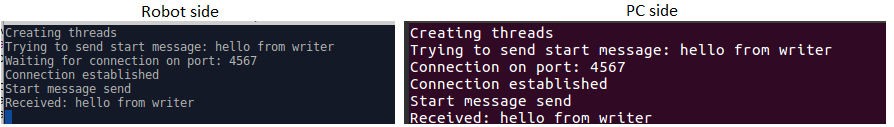
\includegraphics[width=1 \textwidth]{wifi_test_samlet.png}
	\captionof{figure}{Terminal skærmbillede efter gennemførsel af test fra projektet "Terminal skærmudklip fra Wifi test"}
	\label{fig:wifi_test_samlet}
\end{figure}

Som det ses prøver skrive funktionen at sende, men det sker ikke før, der er oprettet forbindelse. 
Lige efter forbindelsen er oprettet, sendes beskeden, som så modtages på modsatte side.
